\documentclass[1p]{elsarticle_modified}
%\bibliographystyle{elsarticle-num}

%\usepackage[colorlinks]{hyperref}
%\usepackage{abbrmath_seonhwa} %\Abb, \Ascr, \Acal ,\Abf, \Afrak
\usepackage{amsfonts}
\usepackage{amssymb}
\usepackage{amsmath}
\usepackage{amsthm}
\usepackage{scalefnt}
\usepackage{amsbsy}
\usepackage{kotex}
\usepackage{caption}
\usepackage{subfig}
\usepackage{color}
\usepackage{graphicx}
\usepackage{xcolor} %% white, black, red, green, blue, cyan, magenta, yellow
\usepackage{float}
\usepackage{setspace}
\usepackage{hyperref}

\usepackage{tikz}
\usetikzlibrary{arrows}

\usepackage{multirow}
\usepackage{array} % fixed length table
\usepackage{hhline}

%%%%%%%%%%%%%%%%%%%%%
\makeatletter
\renewcommand*\env@matrix[1][\arraystretch]{%
	\edef\arraystretch{#1}%
	\hskip -\arraycolsep
	\let\@ifnextchar\new@ifnextchar
	\array{*\c@MaxMatrixCols c}}
\makeatother %https://tex.stackexchange.com/questions/14071/how-can-i-increase-the-line-spacing-in-a-matrix
%%%%%%%%%%%%%%%

\usepackage[normalem]{ulem}

\newcommand{\msout}[1]{\ifmmode\text{\sout{\ensuremath{#1}}}\else\sout{#1}\fi}
%SOURCE: \msout is \stkout macro in https://tex.stackexchange.com/questions/20609/strikeout-in-math-mode

\newcommand{\cancel}[1]{
	\ifmmode
	{\color{red}\msout{#1}}
	\else
	{\color{red}\sout{#1}}
	\fi
}

\newcommand{\add}[1]{
	{\color{blue}\uwave{#1}}
}

\newcommand{\replace}[2]{
	\ifmmode
	{\color{red}\msout{#1}}{\color{blue}\uwave{#2}}
	\else
	{\color{red}\sout{#1}}{\color{blue}\uwave{#2}}
	\fi
}

\newcommand{\Sol}{\mathcal{S}} %segment
\newcommand{\D}{D} %diagram
\newcommand{\A}{\mathcal{A}} %arc


%%%%%%%%%%%%%%%%%%%%%%%%%%%%%5 test

\def\sl{\operatorname{\textup{SL}}(2,\Cbb)}
\def\psl{\operatorname{\textup{PSL}}(2,\Cbb)}
\def\quan{\mkern 1mu \triangleright \mkern 1mu}

\theoremstyle{definition}
\newtheorem{thm}{Theorem}[section]
\newtheorem{prop}[thm]{Proposition}
\newtheorem{lem}[thm]{Lemma}
\newtheorem{ques}[thm]{Question}
\newtheorem{cor}[thm]{Corollary}
\newtheorem{defn}[thm]{Definition}
\newtheorem{exam}[thm]{Example}
\newtheorem{rmk}[thm]{Remark}
\newtheorem{alg}[thm]{Algorithm}

\newcommand{\I}{\sqrt{-1}}
\begin{document}

%\begin{frontmatter}
%
%\title{Boundary parabolic representations of knots up to 8 crossings}
%
%%% Group authors per affiliation:
%\author{Yunhi Cho} 
%\address{Department of Mathematics, University of Seoul, Seoul, Korea}
%\ead{yhcho@uos.ac.kr}
%
%
%\author{Seonhwa Kim} %\fnref{s_kim}}
%\address{Center for Geometry and Physics, Institute for Basic Science, Pohang, 37673, Korea}
%\ead{ryeona17@ibs.re.kr}
%
%\author{Hyuk Kim}
%\address{Department of Mathematical Sciences, Seoul National University, Seoul 08826, Korea}
%\ead{hyukkim@snu.ac.kr}
%
%\author{Seokbeom Yoon}
%\address{Department of Mathematical Sciences, Seoul National University, Seoul, 08826,  Korea}
%\ead{sbyoon15@snu.ac.kr}
%
%\begin{abstract}
%We find all boundary parabolic representation of knots up to 8 crossings.
%
%\end{abstract}
%\begin{keyword}
%    \MSC[2010] 57M25 
%\end{keyword}
%
%\end{frontmatter}

%\linenumbers
%\tableofcontents
%
\newcommand\colored[1]{\textcolor{white}{\rule[-0.35ex]{0.8em}{1.4ex}}\kern-0.8em\color{red} #1}%
%\newcommand\colored[1]{\textcolor{white}{ #1}\kern-2.17ex	\textcolor{white}{ #1}\kern-1.81ex	\textcolor{white}{ #1}\kern-2.15ex\color{red}#1	}

{\Large $\underline{12n_{0796}~(K12n_{0796})}$}

\setlength{\tabcolsep}{10pt}
\renewcommand{\arraystretch}{1.6}
\vspace{1cm}\begin{tabular}{m{100pt}>{\centering\arraybackslash}m{274pt}}
\multirow{5}{120pt}{
	\centering
	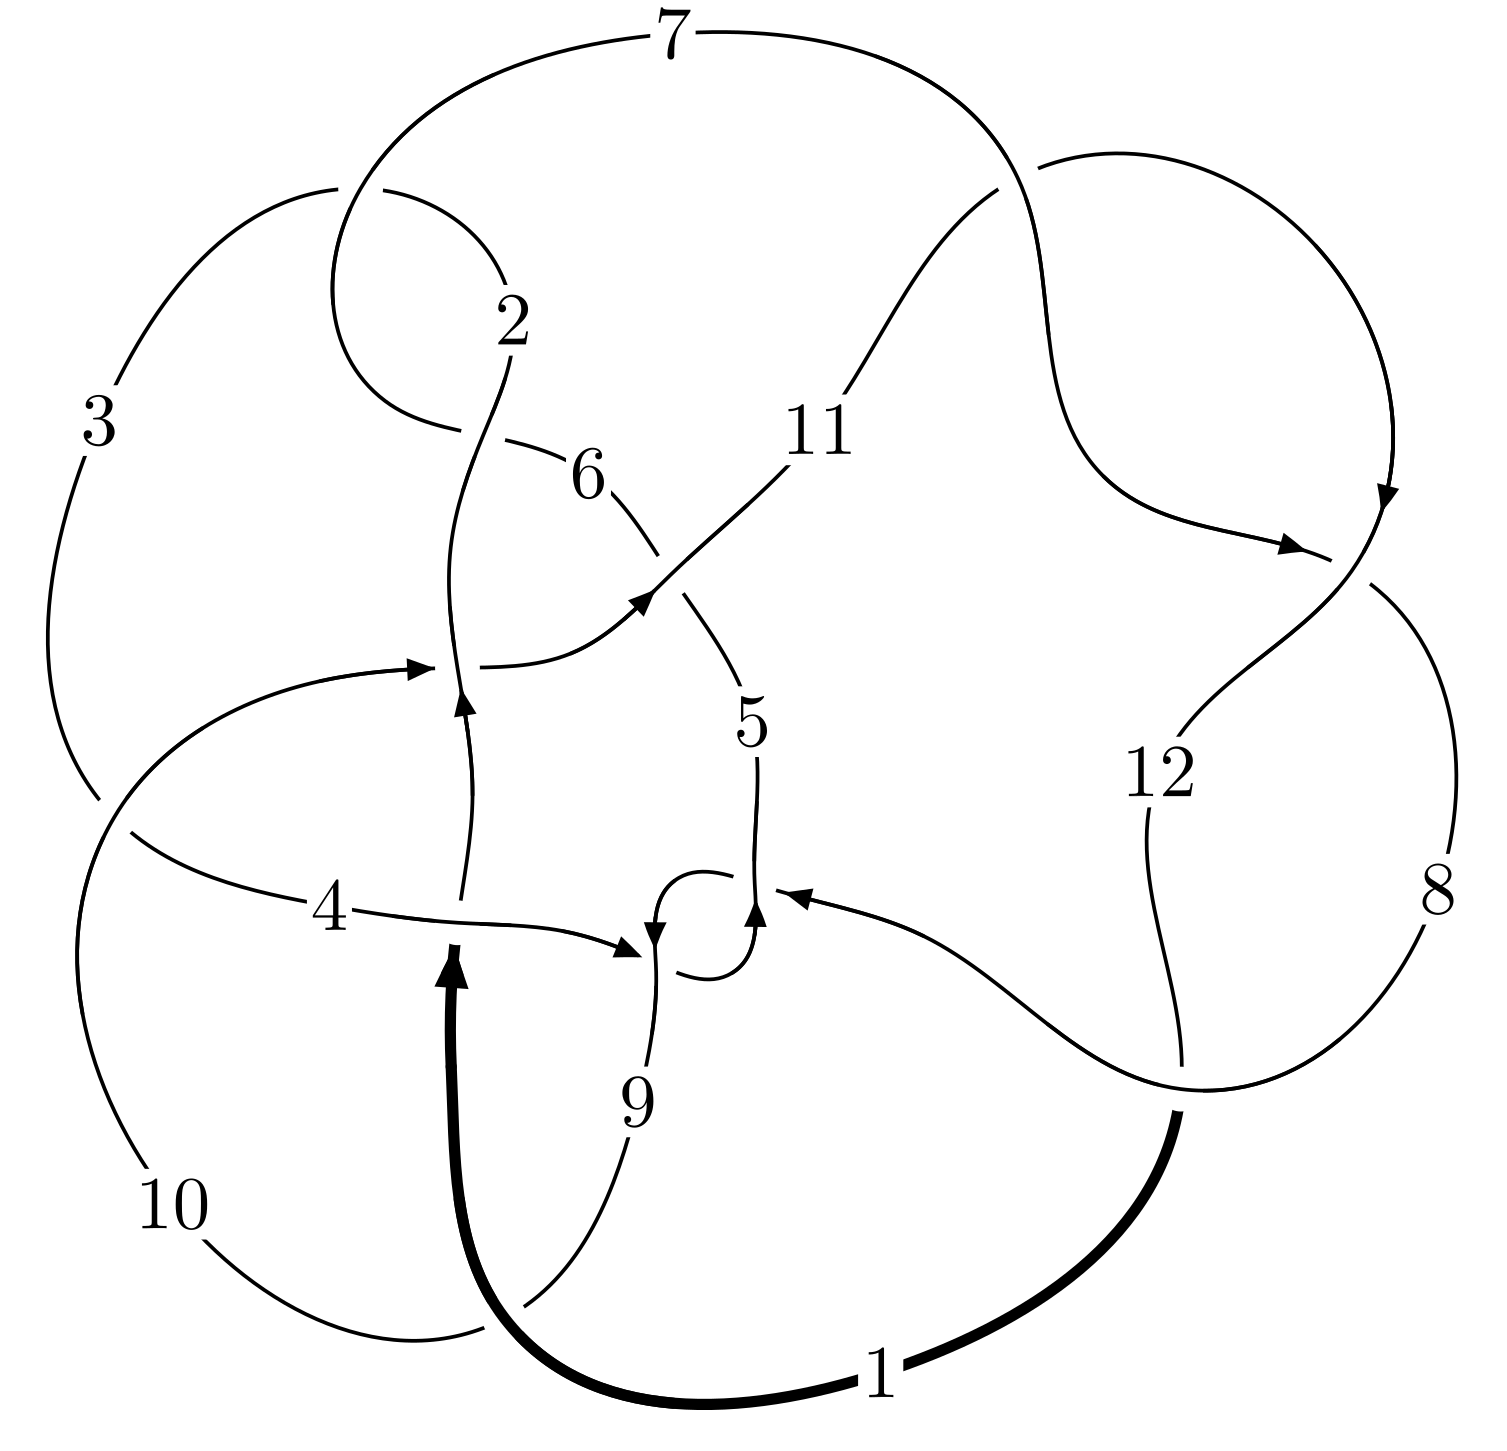
\includegraphics[width=112pt]{../../../GIT/diagram.site/Diagrams/png/2885_12n_0796.png}\\
\ \ \ A knot diagram\footnotemark}&
\allowdisplaybreaks
\textbf{Linearized knot diagam} \\
\cline{2-2}
 &
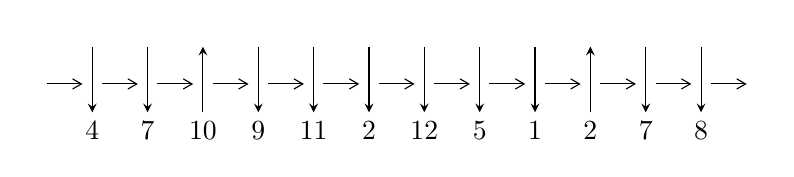
\begin{tikzpicture}[x=20pt, y=17pt]
	% nodes
	\node (C0) at (0, 0) {};
	\node (C1) at (1, 0) {};
	\node (C1U) at (1, +1) {};
	\node (C1D) at (1, -1) {4};

	\node (C2) at (2, 0) {};
	\node (C2U) at (2, +1) {};
	\node (C2D) at (2, -1) {7};

	\node (C3) at (3, 0) {};
	\node (C3U) at (3, +1) {};
	\node (C3D) at (3, -1) {10};

	\node (C4) at (4, 0) {};
	\node (C4U) at (4, +1) {};
	\node (C4D) at (4, -1) {9};

	\node (C5) at (5, 0) {};
	\node (C5U) at (5, +1) {};
	\node (C5D) at (5, -1) {11};

	\node (C6) at (6, 0) {};
	\node (C6U) at (6, +1) {};
	\node (C6D) at (6, -1) {2};

	\node (C7) at (7, 0) {};
	\node (C7U) at (7, +1) {};
	\node (C7D) at (7, -1) {12};

	\node (C8) at (8, 0) {};
	\node (C8U) at (8, +1) {};
	\node (C8D) at (8, -1) {5};

	\node (C9) at (9, 0) {};
	\node (C9U) at (9, +1) {};
	\node (C9D) at (9, -1) {1};

	\node (C10) at (10, 0) {};
	\node (C10U) at (10, +1) {};
	\node (C10D) at (10, -1) {2};

	\node (C11) at (11, 0) {};
	\node (C11U) at (11, +1) {};
	\node (C11D) at (11, -1) {7};

	\node (C12) at (12, 0) {};
	\node (C12U) at (12, +1) {};
	\node (C12D) at (12, -1) {8};
	\node (C13) at (13, 0) {};

	% arrows
	\draw[->,>={angle 60}]
	(C0) edge (C1) (C1) edge (C2) (C2) edge (C3) (C3) edge (C4) (C4) edge (C5) (C5) edge (C6) (C6) edge (C7) (C7) edge (C8) (C8) edge (C9) (C9) edge (C10) (C10) edge (C11) (C11) edge (C12) (C12) edge (C13) ;	\draw[->,>=stealth]
	(C1U) edge (C1D) (C2U) edge (C2D) (C3D) edge (C3U) (C4U) edge (C4D) (C5U) edge (C5D) (C6U) edge (C6D) (C7U) edge (C7D) (C8U) edge (C8D) (C9U) edge (C9D) (C10D) edge (C10U) (C11U) edge (C11D) (C12U) edge (C12D) ;
	\end{tikzpicture} \\
\hhline{~~} \\& 
\textbf{Solving Sequence} \\ \cline{2-2} 
 &
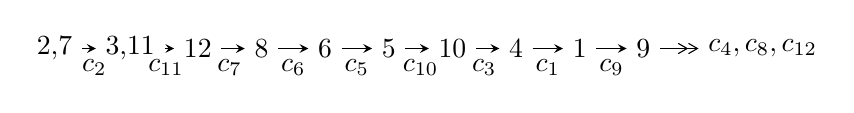
\begin{tikzpicture}[x=23pt, y=7pt]
	% node
	\node (A0) at (-1/8, 0) {2,7};
	\node (A1) at (17/16, 0) {3,11};
	\node (A2) at (17/8, 0) {12};
	\node (A3) at (25/8, 0) {8};
	\node (A4) at (33/8, 0) {6};
	\node (A5) at (41/8, 0) {5};
	\node (A6) at (49/8, 0) {10};
	\node (A7) at (57/8, 0) {4};
	\node (A8) at (65/8, 0) {1};
	\node (A9) at (73/8, 0) {9};
	\node (C1) at (1/2, -1) {$c_{2}$};
	\node (C2) at (13/8, -1) {$c_{11}$};
	\node (C3) at (21/8, -1) {$c_{7}$};
	\node (C4) at (29/8, -1) {$c_{6}$};
	\node (C5) at (37/8, -1) {$c_{5}$};
	\node (C6) at (45/8, -1) {$c_{10}$};
	\node (C7) at (53/8, -1) {$c_{3}$};
	\node (C8) at (61/8, -1) {$c_{1}$};
	\node (C9) at (69/8, -1) {$c_{9}$};
	\node (A10) at (11, 0) {$c_{4},c_{8},c_{12}$};

	% edge
	\draw[->,>=stealth]	
	(A0) edge (A1) (A1) edge (A2) (A2) edge (A3) (A3) edge (A4) (A4) edge (A5) (A5) edge (A6) (A6) edge (A7) (A7) edge (A8) (A8) edge (A9) ;
	\draw[->>,>={angle 60}]	
	(A9) edge (A10);
\end{tikzpicture} \\ 

\end{tabular} \\

\footnotetext{
The image of knot diagram is generated by the software ``\textbf{Draw programme}" developed by Andrew Bartholomew(\url{http://www.layer8.co.uk/maths/draw/index.htm\#Running-draw}), where we modified some parts for our purpose(\url{https://github.com/CATsTAILs/LinksPainter}).
}\phantom \\ \newline 
\centering \textbf{Ideals for irreducible components\footnotemark of $X_{\text{par}}$} 
 
\begin{align*}
I^u_{1}&=\langle 
1.55932\times10^{237} u^{68}+4.63994\times10^{237} u^{67}+\cdots+4.94979\times10^{240} b+1.30744\times10^{242},\\
\phantom{I^u_{1}}&\phantom{= \langle  }7.84763\times10^{240} u^{68}-1.52555\times10^{241} u^{67}+\cdots+8.51859\times10^{243} a+7.61648\times10^{244},\\
\phantom{I^u_{1}}&\phantom{= \langle  }u^{69}-2 u^{68}+\cdots+5609 u+1721\rangle \\
I^u_{2}&=\langle 
-1472105 u^{20}+1018220 u^{19}+\cdots+1155956 b-2256995,\\
\phantom{I^u_{2}}&\phantom{= \langle  }969434 u^{20}-866657 u^{19}+\cdots+1155956 a-2244463,\;u^{21}- u^{20}+\cdots+u-1\rangle \\
\\
\end{align*}
\raggedright * 2 irreducible components of $\dim_{\mathbb{C}}=0$, with total 90 representations.\\
\footnotetext{All coefficients of polynomials are rational numbers. But the coefficients are sometimes approximated in decimal forms when there is not enough margin.}
\newpage
\renewcommand{\arraystretch}{1}
\centering \section*{I. $I^u_{1}= \langle 1.56\times10^{237} u^{68}+4.64\times10^{237} u^{67}+\cdots+4.95\times10^{240} b+1.31\times10^{242},\;7.85\times10^{240} u^{68}-1.53\times10^{241} u^{67}+\cdots+8.52\times10^{243} a+7.62\times10^{244},\;u^{69}-2 u^{68}+\cdots+5609 u+1721 \rangle$}
\flushleft \textbf{(i) Arc colorings}\\
\begin{tabular}{m{7pt} m{180pt} m{7pt} m{180pt} }
\flushright $a_{2}=$&$\begin{pmatrix}1\\0\end{pmatrix}$ \\
\flushright $a_{7}=$&$\begin{pmatrix}0\\u\end{pmatrix}$ \\
\flushright $a_{3}=$&$\begin{pmatrix}1\\u^2\end{pmatrix}$ \\
\flushright $a_{11}=$&$\begin{pmatrix}-0.000921236 u^{68}+0.00179085 u^{67}+\cdots-43.1069 u-8.94101\\-0.000315028 u^{68}-0.000937401 u^{67}+\cdots-31.1935 u-26.4140\end{pmatrix}$ \\
\flushright $a_{12}=$&$\begin{pmatrix}-0.000921236 u^{68}+0.00179085 u^{67}+\cdots-43.1069 u-8.94101\\-0.000404125 u^{68}-0.00110399 u^{67}+\cdots-29.3185 u-26.3252\end{pmatrix}$ \\
\flushright $a_{8}=$&$\begin{pmatrix}0.000650255 u^{68}-0.00261630 u^{67}+\cdots-27.0684 u-14.1292\\0.00264634 u^{68}-0.00616524 u^{67}+\cdots+51.9013 u-0.182253\end{pmatrix}$ \\
\flushright $a_{6}=$&$\begin{pmatrix}u\\u\end{pmatrix}$ \\
\flushright $a_{5}=$&$\begin{pmatrix}0.00238017 u^{68}-0.00420828 u^{67}+\cdots+72.7085 u+11.6824\\-0.00160834 u^{68}+0.00384638 u^{67}+\cdots-14.9392 u+5.56054\end{pmatrix}$ \\
\flushright $a_{10}=$&$\begin{pmatrix}-0.000606208 u^{68}+0.00272825 u^{67}+\cdots-11.9134 u+17.4730\\-0.000315028 u^{68}-0.000937401 u^{67}+\cdots-31.1935 u-26.4140\end{pmatrix}$ \\
\flushright $a_{4}=$&$\begin{pmatrix}0.00315336 u^{68}-0.00460678 u^{67}+\cdots+75.7131 u+28.1976\\-0.00117961 u^{68}+0.00385784 u^{67}+\cdots+8.86048 u+21.3205\end{pmatrix}$ \\
\flushright $a_{1}=$&$\begin{pmatrix}-0.00370793 u^{68}+0.00810308 u^{67}+\cdots-52.0777 u-5.15730\\-0.00114283 u^{68}+0.000233290 u^{67}+\cdots-63.0317 u-36.7696\end{pmatrix}$ \\
\flushright $a_{9}=$&$\begin{pmatrix}0.00335059 u^{68}-0.00924250 u^{67}+\cdots+29.6036 u-19.7274\\0.00574565 u^{68}-0.0116910 u^{67}+\cdots+104.318 u+9.12336\end{pmatrix}$\\&\end{tabular}
\flushleft \textbf{(ii) Obstruction class $= -1$}\\~\\
\flushleft \textbf{(iii) Cusp Shapes $= -0.00547948 u^{68}+0.0175300 u^{67}+\cdots-64.8102 u+67.4117$}\\~\\
\newpage\renewcommand{\arraystretch}{1}
\flushleft \textbf{(iv) u-Polynomials at the component}\newline \\
\begin{tabular}{m{50pt}|m{274pt}}
Crossings & \hspace{64pt}u-Polynomials at each crossing \\
\hline $$\begin{aligned}c_{1}\end{aligned}$$&$\begin{aligned}
&u^{69}-9 u^{68}+\cdots+1142 u-73
\end{aligned}$\\
\hline $$\begin{aligned}c_{2},c_{6}\end{aligned}$$&$\begin{aligned}
&u^{69}-2 u^{68}+\cdots+5609 u+1721
\end{aligned}$\\
\hline $$\begin{aligned}c_{3}\end{aligned}$$&$\begin{aligned}
&u^{69}-9 u^{67}+\cdots+7145 u+559
\end{aligned}$\\
\hline $$\begin{aligned}c_{4},c_{8}\end{aligned}$$&$\begin{aligned}
&u^{69}+3 u^{68}+\cdots+20 u+4
\end{aligned}$\\
\hline $$\begin{aligned}c_{5}\end{aligned}$$&$\begin{aligned}
&u^{69}+u^{68}+\cdots-1168 u+437
\end{aligned}$\\
\hline $$\begin{aligned}c_{7},c_{11},c_{12}\end{aligned}$$&$\begin{aligned}
&u^{69}-2 u^{68}+\cdots+225 u+161
\end{aligned}$\\
\hline $$\begin{aligned}c_{9}\end{aligned}$$&$\begin{aligned}
&u^{69}+6 u^{68}+\cdots-59 u+19
\end{aligned}$\\
\hline $$\begin{aligned}c_{10}\end{aligned}$$&$\begin{aligned}
&u^{69}-38 u^{67}+\cdots+3400 u+644
\end{aligned}$\\
\hline
\end{tabular}\\~\\
\newpage\renewcommand{\arraystretch}{1}
\flushleft \textbf{(v) Riley Polynomials at the component}\newline \\
\begin{tabular}{m{50pt}|m{274pt}}
Crossings & \hspace{64pt}Riley Polynomials at each crossing \\
\hline $$\begin{aligned}c_{1}\end{aligned}$$&$\begin{aligned}
&y^{69}+25 y^{68}+\cdots+523064 y-5329
\end{aligned}$\\
\hline $$\begin{aligned}c_{2},c_{6}\end{aligned}$$&$\begin{aligned}
&y^{69}+70 y^{68}+\cdots-122107391 y-2961841
\end{aligned}$\\
\hline $$\begin{aligned}c_{3}\end{aligned}$$&$\begin{aligned}
&y^{69}-18 y^{68}+\cdots+16869293 y-312481
\end{aligned}$\\
\hline $$\begin{aligned}c_{4},c_{8}\end{aligned}$$&$\begin{aligned}
&y^{69}+43 y^{68}+\cdots-4352 y-16
\end{aligned}$\\
\hline $$\begin{aligned}c_{5}\end{aligned}$$&$\begin{aligned}
&y^{69}+91 y^{68}+\cdots-22307192 y-190969
\end{aligned}$\\
\hline $$\begin{aligned}c_{7},c_{11},c_{12}\end{aligned}$$&$\begin{aligned}
&y^{69}-64 y^{68}+\cdots-149015 y-25921
\end{aligned}$\\
\hline $$\begin{aligned}c_{9}\end{aligned}$$&$\begin{aligned}
&y^{69}+2 y^{68}+\cdots-9629 y-361
\end{aligned}$\\
\hline $$\begin{aligned}c_{10}\end{aligned}$$&$\begin{aligned}
&y^{69}-76 y^{68}+\cdots+45637904 y-414736
\end{aligned}$\\
\hline
\end{tabular}\\~\\
\newpage\flushleft \textbf{(vi) Complex Volumes and Cusp Shapes}
$$\begin{array}{c|c|c}  
\text{Solutions to }I^u_{1}& \I (\text{vol} + \sqrt{-1}CS) & \text{Cusp shape}\\
 \hline 
\begin{aligned}
u &= -0.158298 + 0.986188 I \\
a &= -0.272064 - 1.303170 I \\
b &= -0.115321 - 1.299330 I\end{aligned}
 & -5.58857 + 2.81982 I & -8.00000 + 0. I\phantom{ +0.000000I} \\ \hline\begin{aligned}
u &= -0.158298 - 0.986188 I \\
a &= -0.272064 + 1.303170 I \\
b &= -0.115321 + 1.299330 I\end{aligned}
 & -5.58857 - 2.81982 I & -8.00000 + 0. I\phantom{ +0.000000I} \\ \hline\begin{aligned}
u &= \phantom{-}0.083642 + 1.056570 I \\
a &= -0.337592 + 1.151720 I \\
b &= -0.02643 + 1.67928 I\end{aligned}
 & -1.73341 - 7.58301 I & \phantom{-0.000000 } 0 \\ \hline\begin{aligned}
u &= \phantom{-}0.083642 - 1.056570 I \\
a &= -0.337592 - 1.151720 I \\
b &= -0.02643 - 1.67928 I\end{aligned}
 & -1.73341 + 7.58301 I & \phantom{-0.000000 } 0 \\ \hline\begin{aligned}
u &= \phantom{-}0.897841 + 0.622401 I \\
a &= -1.013910 + 0.791688 I \\
b &= -0.926980 + 0.100178 I\end{aligned}
 & -3.24604 - 2.07530 I & \phantom{-0.000000 } 0 \\ \hline\begin{aligned}
u &= \phantom{-}0.897841 - 0.622401 I \\
a &= -1.013910 - 0.791688 I \\
b &= -0.926980 - 0.100178 I\end{aligned}
 & -3.24604 + 2.07530 I & \phantom{-0.000000 } 0 \\ \hline\begin{aligned}
u &= -0.873469 + 0.076955 I \\
a &= \phantom{-}0.183288 + 0.285846 I \\
b &= -0.406670 - 0.103429 I\end{aligned}
 & -1.062540 + 0.145716 I & -4.45967 + 4.12515 I \\ \hline\begin{aligned}
u &= -0.873469 - 0.076955 I \\
a &= \phantom{-}0.183288 - 0.285846 I \\
b &= -0.406670 + 0.103429 I\end{aligned}
 & -1.062540 - 0.145716 I & -4.45967 - 4.12515 I \\ \hline\begin{aligned}
u &= -0.276545 + 1.134330 I \\
a &= -0.419440 - 1.000890 I \\
b &= -2.15654 - 0.20349 I\end{aligned}
 & \phantom{-}5.65453 + 1.08327 I & \phantom{-0.000000 } 0 \\ \hline\begin{aligned}
u &= -0.276545 - 1.134330 I \\
a &= -0.419440 + 1.000890 I \\
b &= -2.15654 + 0.20349 I\end{aligned}
 & \phantom{-}5.65453 - 1.08327 I & \phantom{-0.000000 } 0\\
 \hline 
 \end{array}$$\newpage$$\begin{array}{c|c|c}  
\text{Solutions to }I^u_{1}& \I (\text{vol} + \sqrt{-1}CS) & \text{Cusp shape}\\
 \hline 
\begin{aligned}
u &= -0.559678 + 0.527322 I \\
a &= -1.39441 - 1.42597 I \\
b &= \phantom{-}0.168662 + 0.071411 I\end{aligned}
 & -7.42057 - 0.68077 I & -9.11367 - 4.86767 I \\ \hline\begin{aligned}
u &= -0.559678 - 0.527322 I \\
a &= -1.39441 + 1.42597 I \\
b &= \phantom{-}0.168662 - 0.071411 I\end{aligned}
 & -7.42057 + 0.68077 I & -9.11367 + 4.86767 I \\ \hline\begin{aligned}
u &= \phantom{-}0.046375 + 0.765714 I \\
a &= \phantom{-}0.29507 + 1.43922 I \\
b &= -0.475537 + 1.205130 I\end{aligned}
 & -2.54675 + 1.17327 I & -8.71427 - 1.88942 I \\ \hline\begin{aligned}
u &= \phantom{-}0.046375 - 0.765714 I \\
a &= \phantom{-}0.29507 - 1.43922 I \\
b &= -0.475537 - 1.205130 I\end{aligned}
 & -2.54675 - 1.17327 I & -8.71427 + 1.88942 I \\ \hline\begin{aligned}
u &= \phantom{-}1.109890 + 0.543098 I \\
a &= -0.167780 - 0.533391 I \\
b &= -0.226182 - 0.061038 I\end{aligned}
 & \phantom{-}2.06906 - 4.86203 I & \phantom{-0.000000 } 0 \\ \hline\begin{aligned}
u &= \phantom{-}1.109890 - 0.543098 I \\
a &= -0.167780 + 0.533391 I \\
b &= -0.226182 + 0.061038 I\end{aligned}
 & \phantom{-}2.06906 + 4.86203 I & \phantom{-0.000000 } 0 \\ \hline\begin{aligned}
u &= -0.275066 + 0.704105 I \\
a &= -0.58805 - 2.16534 I \\
b &= -0.790942 - 0.769428 I\end{aligned}
 & -4.81193 + 0.89227 I & -9.11144 + 1.07907 I \\ \hline\begin{aligned}
u &= -0.275066 - 0.704105 I \\
a &= -0.58805 + 2.16534 I \\
b &= -0.790942 + 0.769428 I\end{aligned}
 & -4.81193 - 0.89227 I & -9.11144 - 1.07907 I \\ \hline\begin{aligned}
u &= \phantom{-}0.353524 + 0.612098 I \\
a &= -1.23670 + 1.80209 I \\
b &= -0.822113 + 0.104555 I\end{aligned}
 & -3.12815 - 2.49344 I & -7.27898 + 4.57610 I \\ \hline\begin{aligned}
u &= \phantom{-}0.353524 - 0.612098 I \\
a &= -1.23670 - 1.80209 I \\
b &= -0.822113 - 0.104555 I\end{aligned}
 & -3.12815 + 2.49344 I & -7.27898 - 4.57610 I\\
 \hline 
 \end{array}$$\newpage$$\begin{array}{c|c|c}  
\text{Solutions to }I^u_{1}& \I (\text{vol} + \sqrt{-1}CS) & \text{Cusp shape}\\
 \hline 
\begin{aligned}
u &= -1.287570 + 0.252312 I \\
a &= -0.798351 - 0.401734 I \\
b &= -0.700910 - 0.154778 I\end{aligned}
 & -3.53458 - 1.35311 I & \phantom{-0.000000 } 0 \\ \hline\begin{aligned}
u &= -1.287570 - 0.252312 I \\
a &= -0.798351 + 0.401734 I \\
b &= -0.700910 + 0.154778 I\end{aligned}
 & -3.53458 + 1.35311 I & \phantom{-0.000000 } 0 \\ \hline\begin{aligned}
u &= \phantom{-}0.438476 + 0.526047 I \\
a &= \phantom{-}1.039740 + 0.065197 I \\
b &= \phantom{-}0.532056 - 0.185656 I\end{aligned}
 & \phantom{-}3.24596 - 0.23179 I & -3.95693 + 3.09799 I \\ \hline\begin{aligned}
u &= \phantom{-}0.438476 - 0.526047 I \\
a &= \phantom{-}1.039740 - 0.065197 I \\
b &= \phantom{-}0.532056 + 0.185656 I\end{aligned}
 & \phantom{-}3.24596 + 0.23179 I & -3.95693 - 3.09799 I \\ \hline\begin{aligned}
u &= \phantom{-}0.331403 + 0.571115 I \\
a &= -0.336557 - 1.133840 I \\
b &= -0.333318 + 0.405393 I\end{aligned}
 & \phantom{-}2.88430 + 3.68981 I & -3.97105 - 4.01517 I \\ \hline\begin{aligned}
u &= \phantom{-}0.331403 - 0.571115 I \\
a &= -0.336557 + 1.133840 I \\
b &= -0.333318 - 0.405393 I\end{aligned}
 & \phantom{-}2.88430 - 3.68981 I & -3.97105 + 4.01517 I \\ \hline\begin{aligned}
u &= \phantom{-}0.003294 + 1.405920 I \\
a &= \phantom{-}0.424182 - 0.124262 I \\
b &= \phantom{-}1.89700 - 0.41536 I\end{aligned}
 & \phantom{-}8.98523 - 1.65207 I & \phantom{-0.000000 } 0 \\ \hline\begin{aligned}
u &= \phantom{-}0.003294 - 1.405920 I \\
a &= \phantom{-}0.424182 + 0.124262 I \\
b &= \phantom{-}1.89700 + 0.41536 I\end{aligned}
 & \phantom{-}8.98523 + 1.65207 I & \phantom{-0.000000 } 0 \\ \hline\begin{aligned}
u &= \phantom{-}1.45256 + 0.09643 I \\
a &= \phantom{-}0.882941 + 0.151010 I \\
b &= \phantom{-}1.014830 - 0.130294 I\end{aligned}
 & -1.63011 - 8.47566 I & \phantom{-0.000000 } 0 \\ \hline\begin{aligned}
u &= \phantom{-}1.45256 - 0.09643 I \\
a &= \phantom{-}0.882941 - 0.151010 I \\
b &= \phantom{-}1.014830 + 0.130294 I\end{aligned}
 & -1.63011 + 8.47566 I & \phantom{-0.000000 } 0\\
 \hline 
 \end{array}$$\newpage$$\begin{array}{c|c|c}  
\text{Solutions to }I^u_{1}& \I (\text{vol} + \sqrt{-1}CS) & \text{Cusp shape}\\
 \hline 
\begin{aligned}
u &= \phantom{-}0.50626 + 1.36552 I \\
a &= -0.571385 + 0.832237 I \\
b &= -1.55177 + 0.45405 I\end{aligned}
 & -0.63369 - 3.48980 I & \phantom{-0.000000 } 0 \\ \hline\begin{aligned}
u &= \phantom{-}0.50626 - 1.36552 I \\
a &= -0.571385 - 0.832237 I \\
b &= -1.55177 - 0.45405 I\end{aligned}
 & -0.63369 + 3.48980 I & \phantom{-0.000000 } 0 \\ \hline\begin{aligned}
u &= \phantom{-}0.304513 + 0.423795 I \\
a &= -1.43929 + 2.57107 I \\
b &= \phantom{-}0.350883 - 0.574081 I\end{aligned}
 & -3.93150 + 6.37374 I & -6.00431 - 0.55984 I \\ \hline\begin{aligned}
u &= \phantom{-}0.304513 - 0.423795 I \\
a &= -1.43929 - 2.57107 I \\
b &= \phantom{-}0.350883 + 0.574081 I\end{aligned}
 & -3.93150 - 6.37374 I & -6.00431 + 0.55984 I \\ \hline\begin{aligned}
u &= -1.45998 + 0.32838 I \\
a &= \phantom{-}0.778216 + 0.237416 I \\
b &= \phantom{-}1.146240 - 0.151845 I\end{aligned}
 & -4.12698 - 1.49086 I & \phantom{-0.000000 } 0 \\ \hline\begin{aligned}
u &= -1.45998 - 0.32838 I \\
a &= \phantom{-}0.778216 - 0.237416 I \\
b &= \phantom{-}1.146240 + 0.151845 I\end{aligned}
 & -4.12698 + 1.49086 I & \phantom{-0.000000 } 0 \\ \hline\begin{aligned}
u &= \phantom{-}0.76152 + 1.29459 I \\
a &= \phantom{-}0.565850 - 0.600524 I \\
b &= \phantom{-}1.73177 - 0.07649 I\end{aligned}
 & \phantom{-}6.56829 - 3.06698 I & \phantom{-0.000000 } 0 \\ \hline\begin{aligned}
u &= \phantom{-}0.76152 - 1.29459 I \\
a &= \phantom{-}0.565850 + 0.600524 I \\
b &= \phantom{-}1.73177 + 0.07649 I\end{aligned}
 & \phantom{-}6.56829 + 3.06698 I & \phantom{-0.000000 } 0 \\ \hline\begin{aligned}
u &= \phantom{-}0.16311 + 1.51940 I \\
a &= -0.278382 + 0.891128 I \\
b &= -1.59418 + 1.00854 I\end{aligned}
 & \phantom{-}3.87490 - 4.93069 I & \phantom{-0.000000 } 0 \\ \hline\begin{aligned}
u &= \phantom{-}0.16311 - 1.51940 I \\
a &= -0.278382 - 0.891128 I \\
b &= -1.59418 - 1.00854 I\end{aligned}
 & \phantom{-}3.87490 + 4.93069 I & \phantom{-0.000000 } 0\\
 \hline 
 \end{array}$$\newpage$$\begin{array}{c|c|c}  
\text{Solutions to }I^u_{1}& \I (\text{vol} + \sqrt{-1}CS) & \text{Cusp shape}\\
 \hline 
\begin{aligned}
u &= \phantom{-}0.11712 + 1.52857 I \\
a &= \phantom{-}0.503854 - 0.260580 I \\
b &= \phantom{-}1.52489 + 0.06927 I\end{aligned}
 & \phantom{-}5.16690 + 0.91358 I & \phantom{-0.000000 } 0 \\ \hline\begin{aligned}
u &= \phantom{-}0.11712 - 1.52857 I \\
a &= \phantom{-}0.503854 + 0.260580 I \\
b &= \phantom{-}1.52489 - 0.06927 I\end{aligned}
 & \phantom{-}5.16690 - 0.91358 I & \phantom{-0.000000 } 0 \\ \hline\begin{aligned}
u &= -0.20757 + 1.56047 I \\
a &= -0.180163 - 0.719584 I \\
b &= -1.35279 - 0.83587 I\end{aligned}
 & \phantom{-}3.38686 + 3.48426 I & \phantom{-0.000000 } 0 \\ \hline\begin{aligned}
u &= -0.20757 - 1.56047 I \\
a &= -0.180163 + 0.719584 I \\
b &= -1.35279 + 0.83587 I\end{aligned}
 & \phantom{-}3.38686 - 3.48426 I & \phantom{-0.000000 } 0 \\ \hline\begin{aligned}
u &= -0.12399 + 1.59477 I \\
a &= \phantom{-}0.681440 + 0.660461 I \\
b &= \phantom{-}1.63144 + 0.20640 I\end{aligned}
 & \phantom{-}8.17838 - 3.00736 I & \phantom{-0.000000 } 0 \\ \hline\begin{aligned}
u &= -0.12399 - 1.59477 I \\
a &= \phantom{-}0.681440 - 0.660461 I \\
b &= \phantom{-}1.63144 - 0.20640 I\end{aligned}
 & \phantom{-}8.17838 + 3.00736 I & \phantom{-0.000000 } 0 \\ \hline\begin{aligned}
u &= \phantom{-}0.06103 + 1.60204 I \\
a &= \phantom{-}0.782383 - 0.156927 I \\
b &= \phantom{-}1.60703 + 0.02690 I\end{aligned}
 & \phantom{-}5.14159 + 1.38074 I & \phantom{-0.000000 } 0 \\ \hline\begin{aligned}
u &= \phantom{-}0.06103 - 1.60204 I \\
a &= \phantom{-}0.782383 + 0.156927 I \\
b &= \phantom{-}1.60703 - 0.02690 I\end{aligned}
 & \phantom{-}5.14159 - 1.38074 I & \phantom{-0.000000 } 0 \\ \hline\begin{aligned}
u &= -0.50160 + 1.56330 I \\
a &= -0.605057 - 0.716082 I \\
b &= -1.51304 - 0.58879 I\end{aligned}
 & \phantom{-}1.18052 + 8.01996 I & \phantom{-0.000000 } 0 \\ \hline\begin{aligned}
u &= -0.50160 - 1.56330 I \\
a &= -0.605057 + 0.716082 I \\
b &= -1.51304 + 0.58879 I\end{aligned}
 & \phantom{-}1.18052 - 8.01996 I & \phantom{-0.000000 } 0\\
 \hline 
 \end{array}$$\newpage$$\begin{array}{c|c|c}  
\text{Solutions to }I^u_{1}& \I (\text{vol} + \sqrt{-1}CS) & \text{Cusp shape}\\
 \hline 
\begin{aligned}
u &= -0.108395 + 0.310529 I \\
a &= \phantom{-}2.04945 - 0.08178 I \\
b &= \phantom{-}0.519163 - 1.201190 I\end{aligned}
 & \phantom{-}1.60702 - 4.33264 I & -3.39028 + 0.73355 I \\ \hline\begin{aligned}
u &= -0.108395 - 0.310529 I \\
a &= \phantom{-}2.04945 + 0.08178 I \\
b &= \phantom{-}0.519163 + 1.201190 I\end{aligned}
 & \phantom{-}1.60702 + 4.33264 I & -3.39028 - 0.73355 I \\ \hline\begin{aligned}
u &= \phantom{-}0.31783 + 1.64373 I \\
a &= -0.410181 - 0.179193 I \\
b &= -1.56558 - 0.16838 I\end{aligned}
 & \phantom{-}9.72300 + 0.50483 I & \phantom{-0.000000 } 0 \\ \hline\begin{aligned}
u &= \phantom{-}0.31783 - 1.64373 I \\
a &= -0.410181 + 0.179193 I \\
b &= -1.56558 + 0.16838 I\end{aligned}
 & \phantom{-}9.72300 - 0.50483 I & \phantom{-0.000000 } 0 \\ \hline\begin{aligned}
u &= -0.112837 + 0.298176 I \\
a &= \phantom{-}1.372770 + 0.307949 I \\
b &= \phantom{-}0.223037 + 0.869700 I\end{aligned}
 & -0.66690 + 1.42409 I & -5.32505 - 6.58254 I \\ \hline\begin{aligned}
u &= -0.112837 - 0.298176 I \\
a &= \phantom{-}1.372770 - 0.307949 I \\
b &= \phantom{-}0.223037 - 0.869700 I\end{aligned}
 & -0.66690 - 1.42409 I & -5.32505 + 6.58254 I \\ \hline\begin{aligned}
u &= -0.312476\phantom{ +0.000000I} \\
a &= \phantom{-}1.51887\phantom{ +0.000000I} \\
b &= -0.349862\phantom{ +0.000000I}\end{aligned}
 & -0.836204\phantom{ +0.000000I} & -10.8240\phantom{ +0.000000I} \\ \hline\begin{aligned}
u &= -0.27602 + 1.70711 I \\
a &= -0.473587 - 0.096462 I \\
b &= -1.57240 - 0.17128 I\end{aligned}
 & \phantom{-}5.92558 + 5.18269 I & \phantom{-0.000000 } 0 \\ \hline\begin{aligned}
u &= -0.27602 - 1.70711 I \\
a &= -0.473587 + 0.096462 I \\
b &= -1.57240 + 0.17128 I\end{aligned}
 & \phantom{-}5.92558 - 5.18269 I & \phantom{-0.000000 } 0 \\ \hline\begin{aligned}
u &= \phantom{-}0.31729 + 1.70235 I \\
a &= \phantom{-}0.215927 - 0.598368 I \\
b &= \phantom{-}1.142090 - 0.229954 I\end{aligned}
 & \phantom{-}4.02110 + 1.66857 I & \phantom{-0.000000 } 0\\
 \hline 
 \end{array}$$\newpage$$\begin{array}{c|c|c}  
\text{Solutions to }I^u_{1}& \I (\text{vol} + \sqrt{-1}CS) & \text{Cusp shape}\\
 \hline 
\begin{aligned}
u &= \phantom{-}0.31729 - 1.70235 I \\
a &= \phantom{-}0.215927 + 0.598368 I \\
b &= \phantom{-}1.142090 + 0.229954 I\end{aligned}
 & \phantom{-}4.02110 - 1.66857 I & \phantom{-0.000000 } 0 \\ \hline\begin{aligned}
u &= \phantom{-}0.26471 + 1.72015 I \\
a &= -0.676450 + 0.114182 I \\
b &= -1.78553 + 0.24731 I\end{aligned}
 & \phantom{-}10.1818 - 10.1391 I & \phantom{-0.000000 } 0 \\ \hline\begin{aligned}
u &= \phantom{-}0.26471 - 1.72015 I \\
a &= -0.676450 - 0.114182 I \\
b &= -1.78553 - 0.24731 I\end{aligned}
 & \phantom{-}10.1818 + 10.1391 I & \phantom{-0.000000 } 0 \\ \hline\begin{aligned}
u &= \phantom{-}0.56884 + 1.65411 I \\
a &= \phantom{-}0.528673 - 0.738965 I \\
b &= \phantom{-}1.73021 - 0.61726 I\end{aligned}
 & \phantom{-}4.1767 - 15.8025 I & \phantom{-0.000000 } 0 \\ \hline\begin{aligned}
u &= \phantom{-}0.56884 - 1.65411 I \\
a &= \phantom{-}0.528673 + 0.738965 I \\
b &= \phantom{-}1.73021 + 0.61726 I\end{aligned}
 & \phantom{-}4.1767 + 15.8025 I & \phantom{-0.000000 } 0 \\ \hline\begin{aligned}
u &= -0.66790 + 1.62331 I \\
a &= \phantom{-}0.490922 + 0.682589 I \\
b &= \phantom{-}1.64092 + 0.46630 I\end{aligned}
 & \phantom{-}0.41185 + 9.31633 I & \phantom{-0.000000 } 0 \\ \hline\begin{aligned}
u &= -0.66790 - 1.62331 I \\
a &= \phantom{-}0.490922 - 0.682589 I \\
b &= \phantom{-}1.64092 - 0.46630 I\end{aligned}
 & \phantom{-}0.41185 - 9.31633 I & \phantom{-0.000000 } 0 \\ \hline\begin{aligned}
u &= -0.05409 + 1.77796 I \\
a &= \phantom{-}0.214954 + 0.777838 I \\
b &= \phantom{-}1.230930 + 0.437174 I\end{aligned}
 & \phantom{-}4.73411 + 4.44269 I & \phantom{-0.000000 } 0 \\ \hline\begin{aligned}
u &= -0.05409 - 1.77796 I \\
a &= \phantom{-}0.214954 - 0.777838 I \\
b &= \phantom{-}1.230930 - 0.437174 I\end{aligned}
 & \phantom{-}4.73411 - 4.44269 I & \phantom{-0.000000 } 0\\
 \hline 
 \end{array}$$\newpage\newpage\renewcommand{\arraystretch}{1}
\centering \section*{II. $I^u_{2}= \langle -1.47\times10^{6} u^{20}+1.02\times10^{6} u^{19}+\cdots+1.16\times10^{6} b-2.26\times10^{6},\;9.69\times10^{5} u^{20}-8.67\times10^{5} u^{19}+\cdots+1.16\times10^{6} a-2.24\times10^{6},\;u^{21}- u^{20}+\cdots+u-1 \rangle$}
\flushleft \textbf{(i) Arc colorings}\\
\begin{tabular}{m{7pt} m{180pt} m{7pt} m{180pt} }
\flushright $a_{2}=$&$\begin{pmatrix}1\\0\end{pmatrix}$ \\
\flushright $a_{7}=$&$\begin{pmatrix}0\\u\end{pmatrix}$ \\
\flushright $a_{3}=$&$\begin{pmatrix}1\\u^2\end{pmatrix}$ \\
\flushright $a_{11}=$&$\begin{pmatrix}-0.838643 u^{20}+0.749732 u^{19}+\cdots-0.873164 u+1.94165\\1.27350 u^{20}-0.880847 u^{19}+\cdots+0.587410 u+1.95249\end{pmatrix}$ \\
\flushright $a_{12}=$&$\begin{pmatrix}-0.838643 u^{20}+0.749732 u^{19}+\cdots-0.873164 u+1.94165\\0.936639 u^{20}-0.594961 u^{19}+\cdots-0.162322 u+1.86358\end{pmatrix}$ \\
\flushright $a_{8}=$&$\begin{pmatrix}1.75994 u^{20}+1.25748 u^{19}+\cdots-8.26896 u+2.95195\\2.45099 u^{20}-0.835356 u^{19}+\cdots-0.576876 u+3.00745\end{pmatrix}$ \\
\flushright $a_{6}=$&$\begin{pmatrix}u\\u\end{pmatrix}$ \\
\flushright $a_{5}=$&$\begin{pmatrix}-1.13843 u^{20}-1.31272 u^{19}+\cdots+8.94957 u-2.96191\\0.218346 u^{20}-0.0130316 u^{19}+\cdots+1.52471 u+0.716223\end{pmatrix}$ \\
\flushright $a_{10}=$&$\begin{pmatrix}-2.11214 u^{20}+1.63058 u^{19}+\cdots-1.46057 u-0.0108412\\1.27350 u^{20}-0.880847 u^{19}+\cdots+0.587410 u+1.95249\end{pmatrix}$ \\
\flushright $a_{4}=$&$\begin{pmatrix}-3.37269 u^{20}+2.25418 u^{19}+\cdots-0.270532 u-1.59771\\0.911568 u^{20}-0.205314 u^{19}+\cdots-0.283777 u+1.12991\end{pmatrix}$ \\
\flushright $a_{1}=$&$\begin{pmatrix}-0.0729249 u^{20}-0.544418 u^{19}+\cdots+1.15694 u-3.07156\\-1.75142 u^{20}+0.273581 u^{19}+\cdots+0.0784632 u-0.836167\end{pmatrix}$ \\
\flushright $a_{9}=$&$\begin{pmatrix}-1.97499 u^{20}+2.56253 u^{19}+\cdots+0.0537434 u-3.30592\\0.305597 u^{20}+0.371861 u^{19}+\cdots-1.77387 u+2.31582\end{pmatrix}$\\&\end{tabular}
\flushleft \textbf{(ii) Obstruction class $= 1$}\\~\\
\flushleft \textbf{(iii) Cusp Shapes $= \frac{3328575}{288989} u^{20}-\frac{3093691}{577978} u^{19}+\cdots+\frac{1150671}{577978} u+\frac{97487}{577978}$}\\~\\
\newpage\renewcommand{\arraystretch}{1}
\flushleft \textbf{(iv) u-Polynomials at the component}\newline \\
\begin{tabular}{m{50pt}|m{274pt}}
Crossings & \hspace{64pt}u-Polynomials at each crossing \\
\hline $$\begin{aligned}c_{1}\end{aligned}$$&$\begin{aligned}
&u^{21}-4 u^{20}+\cdots+4 u-1
\end{aligned}$\\
\hline $$\begin{aligned}c_{2}\end{aligned}$$&$\begin{aligned}
&u^{21}- u^{20}+\cdots+u-1
\end{aligned}$\\
\hline $$\begin{aligned}c_{3}\end{aligned}$$&$\begin{aligned}
&u^{21}+u^{20}+\cdots+13 u+9
\end{aligned}$\\
\hline $$\begin{aligned}c_{4}\end{aligned}$$&$\begin{aligned}
&u^{21}+2 u^{20}+\cdots+8 u+4
\end{aligned}$\\
\hline $$\begin{aligned}c_{5}\end{aligned}$$&$\begin{aligned}
&u^{21}+7 u^{19}+\cdots+30 u+1
\end{aligned}$\\
\hline $$\begin{aligned}c_{6}\end{aligned}$$&$\begin{aligned}
&u^{21}+u^{20}+\cdots+u+1
\end{aligned}$\\
\hline $$\begin{aligned}c_{7}\end{aligned}$$&$\begin{aligned}
&u^{21}- u^{20}+\cdots+5 u-1
\end{aligned}$\\
\hline $$\begin{aligned}c_{8}\end{aligned}$$&$\begin{aligned}
&u^{21}-2 u^{20}+\cdots+8 u-4
\end{aligned}$\\
\hline $$\begin{aligned}c_{9}\end{aligned}$$&$\begin{aligned}
&u^{21}+u^{20}+\cdots-3 u-1
\end{aligned}$\\
\hline $$\begin{aligned}c_{10}\end{aligned}$$&$\begin{aligned}
&u^{21}-3 u^{20}+\cdots+12 u-4
\end{aligned}$\\
\hline $$\begin{aligned}c_{11},c_{12}\end{aligned}$$&$\begin{aligned}
&u^{21}+u^{20}+\cdots+5 u+1
\end{aligned}$\\
\hline
\end{tabular}\\~\\
\newpage\renewcommand{\arraystretch}{1}
\flushleft \textbf{(v) Riley Polynomials at the component}\newline \\
\begin{tabular}{m{50pt}|m{274pt}}
Crossings & \hspace{64pt}Riley Polynomials at each crossing \\
\hline $$\begin{aligned}c_{1}\end{aligned}$$&$\begin{aligned}
&y^{21}+8 y^{20}+\cdots-4 y-1
\end{aligned}$\\
\hline $$\begin{aligned}c_{2},c_{6}\end{aligned}$$&$\begin{aligned}
&y^{21}+13 y^{20}+\cdots+9 y-1
\end{aligned}$\\
\hline $$\begin{aligned}c_{3}\end{aligned}$$&$\begin{aligned}
&y^{21}-3 y^{20}+\cdots-83 y-81
\end{aligned}$\\
\hline $$\begin{aligned}c_{4},c_{8}\end{aligned}$$&$\begin{aligned}
&y^{21}+14 y^{20}+\cdots-112 y-16
\end{aligned}$\\
\hline $$\begin{aligned}c_{5}\end{aligned}$$&$\begin{aligned}
&y^{21}+14 y^{20}+\cdots+864 y-1
\end{aligned}$\\
\hline $$\begin{aligned}c_{7},c_{11},c_{12}\end{aligned}$$&$\begin{aligned}
&y^{21}-25 y^{20}+\cdots+9 y-1
\end{aligned}$\\
\hline $$\begin{aligned}c_{9}\end{aligned}$$&$\begin{aligned}
&y^{21}-3 y^{20}+\cdots- y-1
\end{aligned}$\\
\hline $$\begin{aligned}c_{10}\end{aligned}$$&$\begin{aligned}
&y^{21}-17 y^{20}+\cdots-64 y-16
\end{aligned}$\\
\hline
\end{tabular}\\~\\
\newpage\flushleft \textbf{(vi) Complex Volumes and Cusp Shapes}
$$\begin{array}{c|c|c}  
\text{Solutions to }I^u_{2}& \I (\text{vol} + \sqrt{-1}CS) & \text{Cusp shape}\\
 \hline 
\begin{aligned}
u &= -0.561157 + 0.901561 I \\
a &= -0.68758 - 1.44240 I \\
b &= -0.590397 - 0.678765 I\end{aligned}
 & -5.00046 + 1.80387 I & -12.21784 - 5.60758 I \\ \hline\begin{aligned}
u &= -0.561157 - 0.901561 I \\
a &= -0.68758 + 1.44240 I \\
b &= -0.590397 + 0.678765 I\end{aligned}
 & -5.00046 - 1.80387 I & -12.21784 + 5.60758 I \\ \hline\begin{aligned}
u &= \phantom{-}0.807360 + 0.286313 I \\
a &= -1.38109 + 0.86594 I \\
b &= -0.587723 + 0.592712 I\end{aligned}
 & -4.40952 + 1.11701 I & -14.5809 - 2.0497 I \\ \hline\begin{aligned}
u &= \phantom{-}0.807360 - 0.286313 I \\
a &= -1.38109 - 0.86594 I \\
b &= -0.587723 - 0.592712 I\end{aligned}
 & -4.40952 - 1.11701 I & -14.5809 + 2.0497 I \\ \hline\begin{aligned}
u &= \phantom{-}0.743753 + 0.239370 I \\
a &= -0.276431 + 0.285848 I \\
b &= \phantom{-}0.508126 + 0.521370 I\end{aligned}
 & -1.33875 + 0.63912 I & -11.08801 - 5.90714 I \\ \hline\begin{aligned}
u &= \phantom{-}0.743753 - 0.239370 I \\
a &= -0.276431 - 0.285848 I \\
b &= \phantom{-}0.508126 - 0.521370 I\end{aligned}
 & -1.33875 - 0.63912 I & -11.08801 + 5.90714 I \\ \hline\begin{aligned}
u &= -0.645247 + 0.396216 I \\
a &= -0.362993 + 0.499905 I \\
b &= \phantom{-}0.171757 + 0.896114 I\end{aligned}
 & \phantom{-}0.95419 + 5.02373 I & -10.96767 - 6.73427 I \\ \hline\begin{aligned}
u &= -0.645247 - 0.396216 I \\
a &= -0.362993 - 0.499905 I \\
b &= \phantom{-}0.171757 - 0.896114 I\end{aligned}
 & \phantom{-}0.95419 - 5.02373 I & -10.96767 + 6.73427 I \\ \hline\begin{aligned}
u &= \phantom{-}1.24638\phantom{ +0.000000I} \\
a &= -0.985958\phantom{ +0.000000I} \\
b &= -1.01348\phantom{ +0.000000I}\end{aligned}
 & -4.18100\phantom{ +0.000000I} & -9.64630\phantom{ +0.000000I} \\ \hline\begin{aligned}
u &= \phantom{-}0.011700 + 1.320960 I \\
a &= \phantom{-}0.316294 - 0.431096 I \\
b &= \phantom{-}1.72321 - 0.15242 I\end{aligned}
 & \phantom{-}7.96622 + 0.10384 I & -4.19566 - 0.46618 I\\
 \hline 
 \end{array}$$\newpage$$\begin{array}{c|c|c}  
\text{Solutions to }I^u_{2}& \I (\text{vol} + \sqrt{-1}CS) & \text{Cusp shape}\\
 \hline 
\begin{aligned}
u &= \phantom{-}0.011700 - 1.320960 I \\
a &= \phantom{-}0.316294 + 0.431096 I \\
b &= \phantom{-}1.72321 + 0.15242 I\end{aligned}
 & \phantom{-}7.96622 - 0.10384 I & -4.19566 + 0.46618 I \\ \hline\begin{aligned}
u &= -0.435613 + 1.277620 I \\
a &= -0.403231 - 0.827190 I \\
b &= -1.96724 - 0.36213 I\end{aligned}
 & \phantom{-}5.47011 + 2.02608 I & -7.19785 - 3.46074 I \\ \hline\begin{aligned}
u &= -0.435613 - 1.277620 I \\
a &= -0.403231 + 0.827190 I \\
b &= -1.96724 + 0.36213 I\end{aligned}
 & \phantom{-}5.47011 - 2.02608 I & -7.19785 + 3.46074 I \\ \hline\begin{aligned}
u &= \phantom{-}0.511370 + 0.359085 I \\
a &= \phantom{-}1.95727 - 1.44685 I \\
b &= -0.377286 - 0.543412 I\end{aligned}
 & -7.65043 + 1.27003 I & -13.8530 - 5.9198 I \\ \hline\begin{aligned}
u &= \phantom{-}0.511370 - 0.359085 I \\
a &= \phantom{-}1.95727 + 1.44685 I \\
b &= -0.377286 + 0.543412 I\end{aligned}
 & -7.65043 - 1.27003 I & -13.8530 + 5.9198 I \\ \hline\begin{aligned}
u &= -0.512008 + 0.216126 I \\
a &= \phantom{-}2.53508 + 0.79978 I \\
b &= \phantom{-}0.013476 - 0.796482 I\end{aligned}
 & -4.42994 + 7.07571 I & -12.1028 - 7.6122 I \\ \hline\begin{aligned}
u &= -0.512008 - 0.216126 I \\
a &= \phantom{-}2.53508 - 0.79978 I \\
b &= \phantom{-}0.013476 + 0.796482 I\end{aligned}
 & -4.42994 - 7.07571 I & -12.1028 + 7.6122 I \\ \hline\begin{aligned}
u &= -0.18694 + 1.62746 I \\
a &= \phantom{-}0.543871 + 0.241555 I \\
b &= \phantom{-}1.41334 - 0.08784 I\end{aligned}
 & \phantom{-}6.13244 - 1.40053 I & -1.40328 + 1.79349 I \\ \hline\begin{aligned}
u &= -0.18694 - 1.62746 I \\
a &= \phantom{-}0.543871 - 0.241555 I \\
b &= \phantom{-}1.41334 + 0.08784 I\end{aligned}
 & \phantom{-}6.13244 + 1.40053 I & -1.40328 - 1.79349 I \\ \hline\begin{aligned}
u &= \phantom{-}0.14359 + 1.63447 I \\
a &= -0.248205 + 0.792792 I \\
b &= -1.30052 + 0.82918 I\end{aligned}
 & \phantom{-}2.75172 - 5.22509 I & -10.06988 + 5.83206 I\\
 \hline 
 \end{array}$$\newpage$$\begin{array}{c|c|c}  
\text{Solutions to }I^u_{2}& \I (\text{vol} + \sqrt{-1}CS) & \text{Cusp shape}\\
 \hline 
\begin{aligned}
u &= \phantom{-}0.14359 - 1.63447 I \\
a &= -0.248205 - 0.792792 I \\
b &= -1.30052 - 0.82918 I\end{aligned}
 & \phantom{-}2.75172 + 5.22509 I & -10.06988 - 5.83206 I\\
 \hline 
 \end{array}$$\newpage
\newpage\renewcommand{\arraystretch}{1}
\centering \section*{ III. u-Polynomials}
\begin{tabular}{m{50pt}|m{274pt}}
Crossings & \hspace{64pt}u-Polynomials at each crossing \\
\hline $$\begin{aligned}c_{1}\end{aligned}$$&$\begin{aligned}
&(u^{21}-4 u^{20}+\cdots+4 u-1)(u^{69}-9 u^{68}+\cdots+1142 u-73)
\end{aligned}$\\
\hline $$\begin{aligned}c_{2}\end{aligned}$$&$\begin{aligned}
&(u^{21}- u^{20}+\cdots+u-1)(u^{69}-2 u^{68}+\cdots+5609 u+1721)
\end{aligned}$\\
\hline $$\begin{aligned}c_{3}\end{aligned}$$&$\begin{aligned}
&(u^{21}+u^{20}+\cdots+13 u+9)(u^{69}-9 u^{67}+\cdots+7145 u+559)
\end{aligned}$\\
\hline $$\begin{aligned}c_{4}\end{aligned}$$&$\begin{aligned}
&(u^{21}+2 u^{20}+\cdots+8 u+4)(u^{69}+3 u^{68}+\cdots+20 u+4)
\end{aligned}$\\
\hline $$\begin{aligned}c_{5}\end{aligned}$$&$\begin{aligned}
&(u^{21}+7 u^{19}+\cdots+30 u+1)(u^{69}+u^{68}+\cdots-1168 u+437)
\end{aligned}$\\
\hline $$\begin{aligned}c_{6}\end{aligned}$$&$\begin{aligned}
&(u^{21}+u^{20}+\cdots+u+1)(u^{69}-2 u^{68}+\cdots+5609 u+1721)
\end{aligned}$\\
\hline $$\begin{aligned}c_{7}\end{aligned}$$&$\begin{aligned}
&(u^{21}- u^{20}+\cdots+5 u-1)(u^{69}-2 u^{68}+\cdots+225 u+161)
\end{aligned}$\\
\hline $$\begin{aligned}c_{8}\end{aligned}$$&$\begin{aligned}
&(u^{21}-2 u^{20}+\cdots+8 u-4)(u^{69}+3 u^{68}+\cdots+20 u+4)
\end{aligned}$\\
\hline $$\begin{aligned}c_{9}\end{aligned}$$&$\begin{aligned}
&(u^{21}+u^{20}+\cdots-3 u-1)(u^{69}+6 u^{68}+\cdots-59 u+19)
\end{aligned}$\\
\hline $$\begin{aligned}c_{10}\end{aligned}$$&$\begin{aligned}
&(u^{21}-3 u^{20}+\cdots+12 u-4)(u^{69}-38 u^{67}+\cdots+3400 u+644)
\end{aligned}$\\
\hline $$\begin{aligned}c_{11},c_{12}\end{aligned}$$&$\begin{aligned}
&(u^{21}+u^{20}+\cdots+5 u+1)(u^{69}-2 u^{68}+\cdots+225 u+161)
\end{aligned}$\\
\hline
\end{tabular}\newpage\renewcommand{\arraystretch}{1}
\centering \section*{ IV. Riley Polynomials}
\begin{tabular}{m{50pt}|m{274pt}}
Crossings & \hspace{64pt}Riley Polynomials at each crossing \\
\hline $$\begin{aligned}c_{1}\end{aligned}$$&$\begin{aligned}
&(y^{21}+8 y^{20}+\cdots-4 y-1)(y^{69}+25 y^{68}+\cdots+523064 y-5329)
\end{aligned}$\\
\hline $$\begin{aligned}c_{2},c_{6}\end{aligned}$$&$\begin{aligned}
&(y^{21}+13 y^{20}+\cdots+9 y-1)\\
&\cdot(y^{69}+70 y^{68}+\cdots-122107391 y-2961841)
\end{aligned}$\\
\hline $$\begin{aligned}c_{3}\end{aligned}$$&$\begin{aligned}
&(y^{21}-3 y^{20}+\cdots-83 y-81)\\
&\cdot(y^{69}-18 y^{68}+\cdots+16869293 y-312481)
\end{aligned}$\\
\hline $$\begin{aligned}c_{4},c_{8}\end{aligned}$$&$\begin{aligned}
&(y^{21}+14 y^{20}+\cdots-112 y-16)(y^{69}+43 y^{68}+\cdots-4352 y-16)
\end{aligned}$\\
\hline $$\begin{aligned}c_{5}\end{aligned}$$&$\begin{aligned}
&(y^{21}+14 y^{20}+\cdots+864 y-1)\\
&\cdot(y^{69}+91 y^{68}+\cdots-22307192 y-190969)
\end{aligned}$\\
\hline $$\begin{aligned}c_{7},c_{11},c_{12}\end{aligned}$$&$\begin{aligned}
&(y^{21}-25 y^{20}+\cdots+9 y-1)(y^{69}-64 y^{68}+\cdots-149015 y-25921)
\end{aligned}$\\
\hline $$\begin{aligned}c_{9}\end{aligned}$$&$\begin{aligned}
&(y^{21}-3 y^{20}+\cdots- y-1)(y^{69}+2 y^{68}+\cdots-9629 y-361)
\end{aligned}$\\
\hline $$\begin{aligned}c_{10}\end{aligned}$$&$\begin{aligned}
&(y^{21}-17 y^{20}+\cdots-64 y-16)\\
&\cdot(y^{69}-76 y^{68}+\cdots+45637904 y-414736)
\end{aligned}$\\
\hline
\end{tabular}
\vskip 2pc
\end{document}